
\chapter{社会契約説}



\section{ホッブズ『リヴァイアサン』 (1651)}




トマス・ホッブズ (Thomas Hobbes, 1588-1679)。

出典:ホッブズ『リヴァイアサン』、永井道雄・宗片邦義訳, 『世界の名著28 ホッブズ』収録, 中央公論社, 1979。




\subsection{人間は本来平等である}



《自然》は人間を心身の諸能力において平等につくった。したがって、時には他の人間よりも明らかに肉体的に強く精神的に機敏な人が見いだされはするが、しかしすべての能力を総合して考えれば、個人差はわずかであり、ある人が要求できない利益を他の人が要求できるほど大きなものではない。たとえば肉体的な強さについていえば、もっとも弱いものでもひそかに陰謀をたくらんだり、自分と同様の危険にさらされているものと共謀することによって、もっとも強いものをも倒すだけの強さを持っている。



また精神的諸能力に関しては、
% 〔ことばにもとづく諸技術、特に学問と呼ばれるところの一般的で誤りのない規則にもとづいてことをすすめる技術{\——}これは少数者が少数のことについて持っているにすぎない。なぜならそれは生得の能力ではなくまた〔深慮のように〕他のものを求めているあいだに習得されるといったものでもない{\——}を除くとすれば〕
肉体的な強さの場合以上の平等を見いだす。



たとえば思慮についても、それは経験にほかならず、等しい時間ある仕事に等しく専念したことについてはすべての人に等しく与えられる。この平等性を信じがたいものとするのは、おそらくは人が自己の知恵についていだく自惚れである。大部分の人間は、自分を自分以外のほんの少数の、名声があるとか自分と意見が一致するとかによって是認している人々を除く他の一般大衆に比べて、自分ははるかに知恵をいだいていると考えている。

つまり多くの人が自分より知力に富み、雄弁で知識があることを認めながらも、しかもなお、自分と同じ程度に賢明な人間が大勢いると信じようとしないのが人間の本性である。自分の知力は手近に、しかし他人のそれは遠くに見る。しかし、これは人間がその点において不平等であるよりは平等であることをむしろ証明している。すべての人がその分け前に満足しているということほど、平等な配分を示す大きなしるしはふつうはない。


  \begin{figure}[htbp]
    \centering
      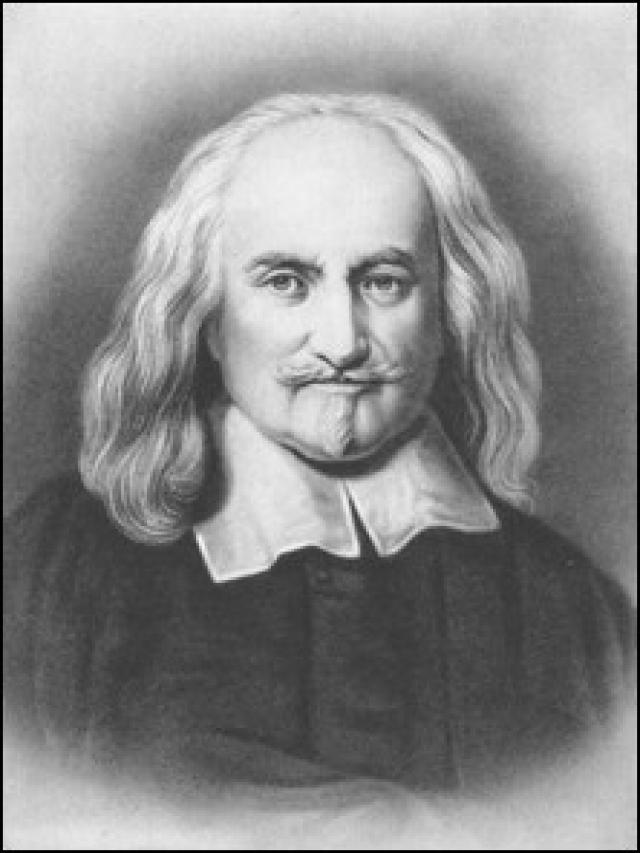
\includegraphics[width=50mm]{images/Thomas-Hobbes2.jpg}
    \caption{ホッブズ}
  \end{figure}



\subsection{平等から他にたいする不信が生じる}


この能力の平等から、目的達成に際しての希望の平等が生じる。それゆえ、もしも二人の者が同一の物を欲求し、それが同時に享受できないものであれば、彼らは敵となり、その目的(として自己保存であるが、ときには快楽のみ)にいたる途上において、たがいに相手をほろぼすか、屈服させようと努める。すなわちつぎのようなことがいえる。侵入者にとって相手の単独の力以外に恐れるもののないところでは、ある人が植え、種子をまき、快適な屋敷をつくりあるいは所有すると、他の人々が力を結合してやってきて、彼の労働の成果だけではなく彼の生命あるいは自由までも奪おうとすることが、おそらく予期されるであろう。そしてその侵入者自身がまた他からの同様な危険にさらされる。




\subsection{不信から戦争が起こる}




このような相互不信から自己を守るには、機先を制するほど適切は方法はない。すなわち力や策によってできるだけすべての人間の身体を、自分をおびやかすほど大きな力がなくなるまで支配することである。それは自己保存に必要な程度のことであり、一般的に許される。



また人によっては、自己の安全のための必要を越えて征服を追及し、征服行為における自己の力を眺めて楽しむ者がある。したがって、もしそのようなことがなければ謙虚に限界のなかで安楽を楽しむであろう他の人々も、侵略によって自己の力を増大させないかぎり、守勢にたつだけでは、長く自己を存続させることができなくなる。であるから、他にたいする支配の増加は自己保存のために必要であり、許されるのが当然である。



また、すべての人間を畏怖させうる権力のないところでは、人間は仲間をつくることになんの喜びも感じない(それどころか、逆にひじょうな悲哀を覚える)。というのは人間はだれしも自己評価と同じ高さの評価を仲間に期待する。そして軽蔑とか過小評価とかのどのようなしるしに出あっても、彼らには害を与え、また他の者にはこれを見せしめにすることによって、彼らからより大きな評価を引き出そうと努力する。〔そしてそれは、双方をしずめる共通の権力がない場合には、たがいに相手を滅亡させるには十分なのである〕



すなわち、人間の本性には、争いについての主要な原因が三つある。第一は、
競争、第二は不信、第三は自負である。



第一の競争は、人々が獲物を得るために、第二の不信は安全を、第三の自負は名声を求めて、いずれも侵略を行なわせる。第一は、他人の人格、妻、子供、家畜の主人となるために、第二は自分を防衛するために、第三は一語、一笑、意見の相違、その他過小評価のしるしになる瑣末事に関して、それらが直接自己の人格に向けられたか、間接に自己の親戚、友人、国民、職業あるいは名称に向けられたかを問わず、やはり暴力を用いさせる。



\subsection{社会状態の外では、各人の各人にたいする戦争状態は常に存在する}


以上によって明らかなことは、自分たちすべてを畏怖させるような共通の権力がないあいだは、人間は戦争と呼ばれる状態、各人の各人にたいする戦争状態にある。なぜなら、《戦争》とは、闘争つまり戦闘行為だけではない。闘争によって争おうとする意志が十分に示されていさえすれば、そのあいだは戦争である。戦争の本質を考察するにはしたがって、天候の本質を考察する場合と同じく「時間」の概念を考慮しなければならない。悪天候とは一度や二度のにわか雨ではなく、雨の降りそうな日が何日も続くことであるように、戦争の本質は実際の戦闘行為にあるのではない。その反対へ向かおうとする保証のまったく見られないあいだのそれへのあきらかな志向が戦争である。その他の期間すべて《平和》である。



\subsection{戦争状態に伴うさまざまの不便}

したがって、各人が各人にとって敵である戦争状態に伴うあらゆることは、自己の力と創意によって得られる以外になんの保証もなしに生きてゆく人々についても同じように伴う。このような状態においては勤労の占める場所はない。勤労の果実が不確実だからである。したがって、土地の耕作も、航海も行なわれず、海路輸入される物資の利用、便利な建物、多くの力を必要とするようなものを運搬し移動する道具、地表面にかんする知識、時間の計算、技術、文字、社会のいずれもない。そして何よりも悪いことに、耐えざる恐怖と、暴力による死の危険がある。そこでは、人間の生活は孤独で貧しく、きたならしく、残忍でしかも短い。……



% こうした事情を十分に考察したことのない人は、自然がこのように人々を分離させ、相互に侵略したり滅ぼしあったりさせるということをふしぎに思うであろう。そして彼は、情念から引き出されたこの推論を信用せず、それが経験によって確認されることを望むであろう。

% そこで彼に、自分に即してつぎのような場合を考えてもらいたい。旅に出るとき、人は武装して、さらに十分な仲間をつれて行きたいと思う。また、睡眠をとるときにはドアに鍵をかける。自分の家のなかですら、金庫に鍵をかける。しかも法律があり武装した公吏がいて、権利侵害がなされた場合にはその復讐をしてくれるということがわかっているのにそうするのである。さらに、人が武装して馬に乗るというのは、自分と同じ国民をどう思っているのか、ドアに鍵をかけるとき自分と同じ市民たちをどう思っているのかを考えてみるがよい。私がことばで行なったと同じように、彼は行為によって、人間を責めているのではないか。

% だからといって、彼も私もそうすることによって人間性を責めているのではない。人間の意欲やその他の情念は、それ自体としてはけっして罪ではない。それらの情念から生じる行為も、それを禁じる法の存在を人が知るまでは罪ではない。そして法が禁じていることは、法がつくられるまでは知りえないし、またいかなる法も、それをつくる人格について人々が同意するまではつくりえない。


% あるいは、

……こうした戦争の時代または状態は一度も存在しなかったと考えられるかもしれない。そして私も、それが一般に全世界にわたって見られたとは信じていない。しかし今日でもそのような生活が行なわれている地方はたくさんある。たとえばアメリカの多くの地方の野蛮民族の場合、たしかに小家族においては自然の情欲にもとづく和合によった統治が見られるけれども、それ以外にはまったく統治は見られない。そして今日でも前述したとおりの残忍な生活法がとられている

いずれにせよ、万人が恐れをいだく共通の力が存在しない場合の生活がどのようなものか。それはかつては平和な統治のもとに暮らしていた人々が内乱によって落ちこむ生活のしかたを考えれば、そこから看取できるであろう。

たとえ、ここの人々がたがいに論争状態にあった時期がまったくなかったとしても、しかもあらゆる時代において王や主権所有人格たちは、その独立性のゆえにたえず嫉妬しあい、たがいに武器を向けあいじっと相手の様子をうかがって、まるで剣闘士の姿勢よろしく身構えてきた。すなわち、王国の国境の要塞、守備兵、銃砲、それに隣国にたいする絶えざるスパイ、これらの存在は戦時体制にほかならない。もっとも、そうすることによって国民の勤労は維持されるから、そのために個々人の自由に伴う悲惨は生まれないのである。


\subsection{戦争状態においては何事も不正ではない}

このような各人の各人にたいする戦争からは、何事も不正ではないということが当然帰結される。正邪とか正義不正義の観念はそこには存在しない。共通の権力が存在しないところに法はなく、法が存在しないところには不正はない。力と\ruby{欺瞞}{ぎまん}は戦争における二つの主要な美徳である。正義と不正義とは肉体と精神のいずれの機能でもない。もしそうであれば、それらは感覚や情念と同じように世界にただひとりでいる人間のなかにも存在するであろう。それらは孤独のなかではなく社会のなかにある人間にかんする性質である。


また前述の状態の必然的結果として、そこには管理権も支配権もなく、「私の物」と「あなたの物」の区別もない。各人が自分で獲得しうる物だけが各人のものであり、しかもそれは、それを保持していることができる期間だけである。



人間が実際にまったくの自然状態におかれたさいの不幸な状態に関しては以上にとどめる。もちろん彼はそこから逸脱しうる可能性を持っており、それは部分的には情念に、部分的には理性による。



\subsection{人々を平和に向かわせる情念}

人々を平和に志向させる情念には、死の恐怖、快適な生活に必要なものを求める意欲、勤労によってそれらを獲得しようとする希望がある。また人間は理性の示唆によって、たがいに同意できるような都合のよい平和のための諸条項を考えだす。そのような諸条項は自然法とも呼ばれる。私はつぎの二章において、それらについてさらに詳しく論じようと思う。




% \subsection*{自然法と契約}



% \section*{自然権とは何か}



\subsection{自然権とは何か}

著作家たちが「Jus Naturale」と一般に呼んでいる《自然権》とは、各人が自分自身の自然すなわち生命を維持するために、自分の力を自分が欲するように用いうるよう各人が持っている自由である。したがって、それは自分自身の判断と理性とにおいて、そのためにもっとも適当な手段であると考えられるあらゆることを行なう自由である。

% \subsection{自由とは何か}

% 《自由》(リバティ)とは、この語の本来の意味に従えば、外的な障害の存在しないことと解される。この障害は、人がその意図することを行なう力の一部をしばしば奪いはするが、彼の判断と理性の命令に従って彼に残された力を行使することを阻止することはできない。

\subsection{自然法とは何か}


《自然法》(Lex Naturalis)とは、理性によって発見された戒律または一般法則であり、それによって人はその生命を破壊したり、生命維持の手段を奪い去るようなことがらを行なったり、また生命がもっともよく維持されると彼が考えることを怠ることが禁じられる。というのは、この問題について論ずる人たちは、よく「ユス」と「レクス」すなわち「権利」(Right)と「法」(Law)を混同するが、それは区別されるべきものである。なぜならば、《権利》はある行為をやったりやらなかったりする自由であり、《法》は、そのどちらかに決定し、それを拘束するものだからである。したがって法と権利には、義務と自由のようなちがいがあり、同一のことがらに関して勝者が一致することはない。

\subsection{自然的には、あらゆる人間があらゆるものに権利を持つ}


そして人間の自然状態は、〔前章に言明したとおり〕各人の各人にたいする戦争状態であり、この場合人が統治されるのはみずからの理性によるのであって、自己の生命をその敵から守り維持するためには、それに役だつもので用いてならないものはない。そこでつぎのようにいうことができる。すなわち、このような状態においては、人はだれでもあらゆるものにたいして、おたがいに相手の身体にたいしてまで権利を持つ。したがって各人の万物にたいするこの自然の権利が存続するかぎり、自然がふつう人間に与えている生きる期間を生き抜くための安全は、いかなる人間にも、〔いかに力強く賢明であろうとも〕まったく保証されてはいない。ゆえにつぎのことは、理性による戒律ないしは一般法則である。「各人は望みのあるかぎり、平和をかちとるように努力すべきである。それが不可能の場合には、戦争によるあらゆる援助と利益を求め、かつこれを用いてもよい」。この法則の第一の部分は、最初の、しかも基本的な自然法を含んでいる。すなわち、「平和を求め、それに従え」。第二の部分には自然権の要約であるが、それは「可能なあらゆる方法によって、自分自身を守れ」である。

\subsection{第二の自然法}



平和のために努力するよう命じたこの基本的自然法から、つぎの第二の法が引きだされる。すなわち、「平和のために、また自己防衛のために必要であると考えられるかぎりにおいて、人は、他の人々も同意するならば、万物にたいするこの権利を喜んで放棄すべきである。そして自分が他の人々にたいして持つ自由は、他の人々が自分にたいして持つことを自分が進んで認めることのできる範囲で満足すべきである」。なぜならば、各人がその好むところを行なう権利を保有しているかぎり、万人は戦争の状態にある。

しかし、もしも他の人々が彼のようにみずからの権利を放棄することを欲しないならば、だれもその権利を放棄すべき理由はない。なぜなら、そのときには自分を平和に向かわせるより、むしろ餌食にさらす〔そうする義務はだれにもない〕ことになるからである。それこをが「福音書」中のあの法である。「すべて自分にしてもらいたいことは、あなた方もそのように人々にせよ」。また、万人の法もそうである。「Quod tibi feiri non vis, alteri ne feceris」(みずからの求めざるところを、他に行なうなかれ)


  \begin{figure}[htbp]
    \centering
      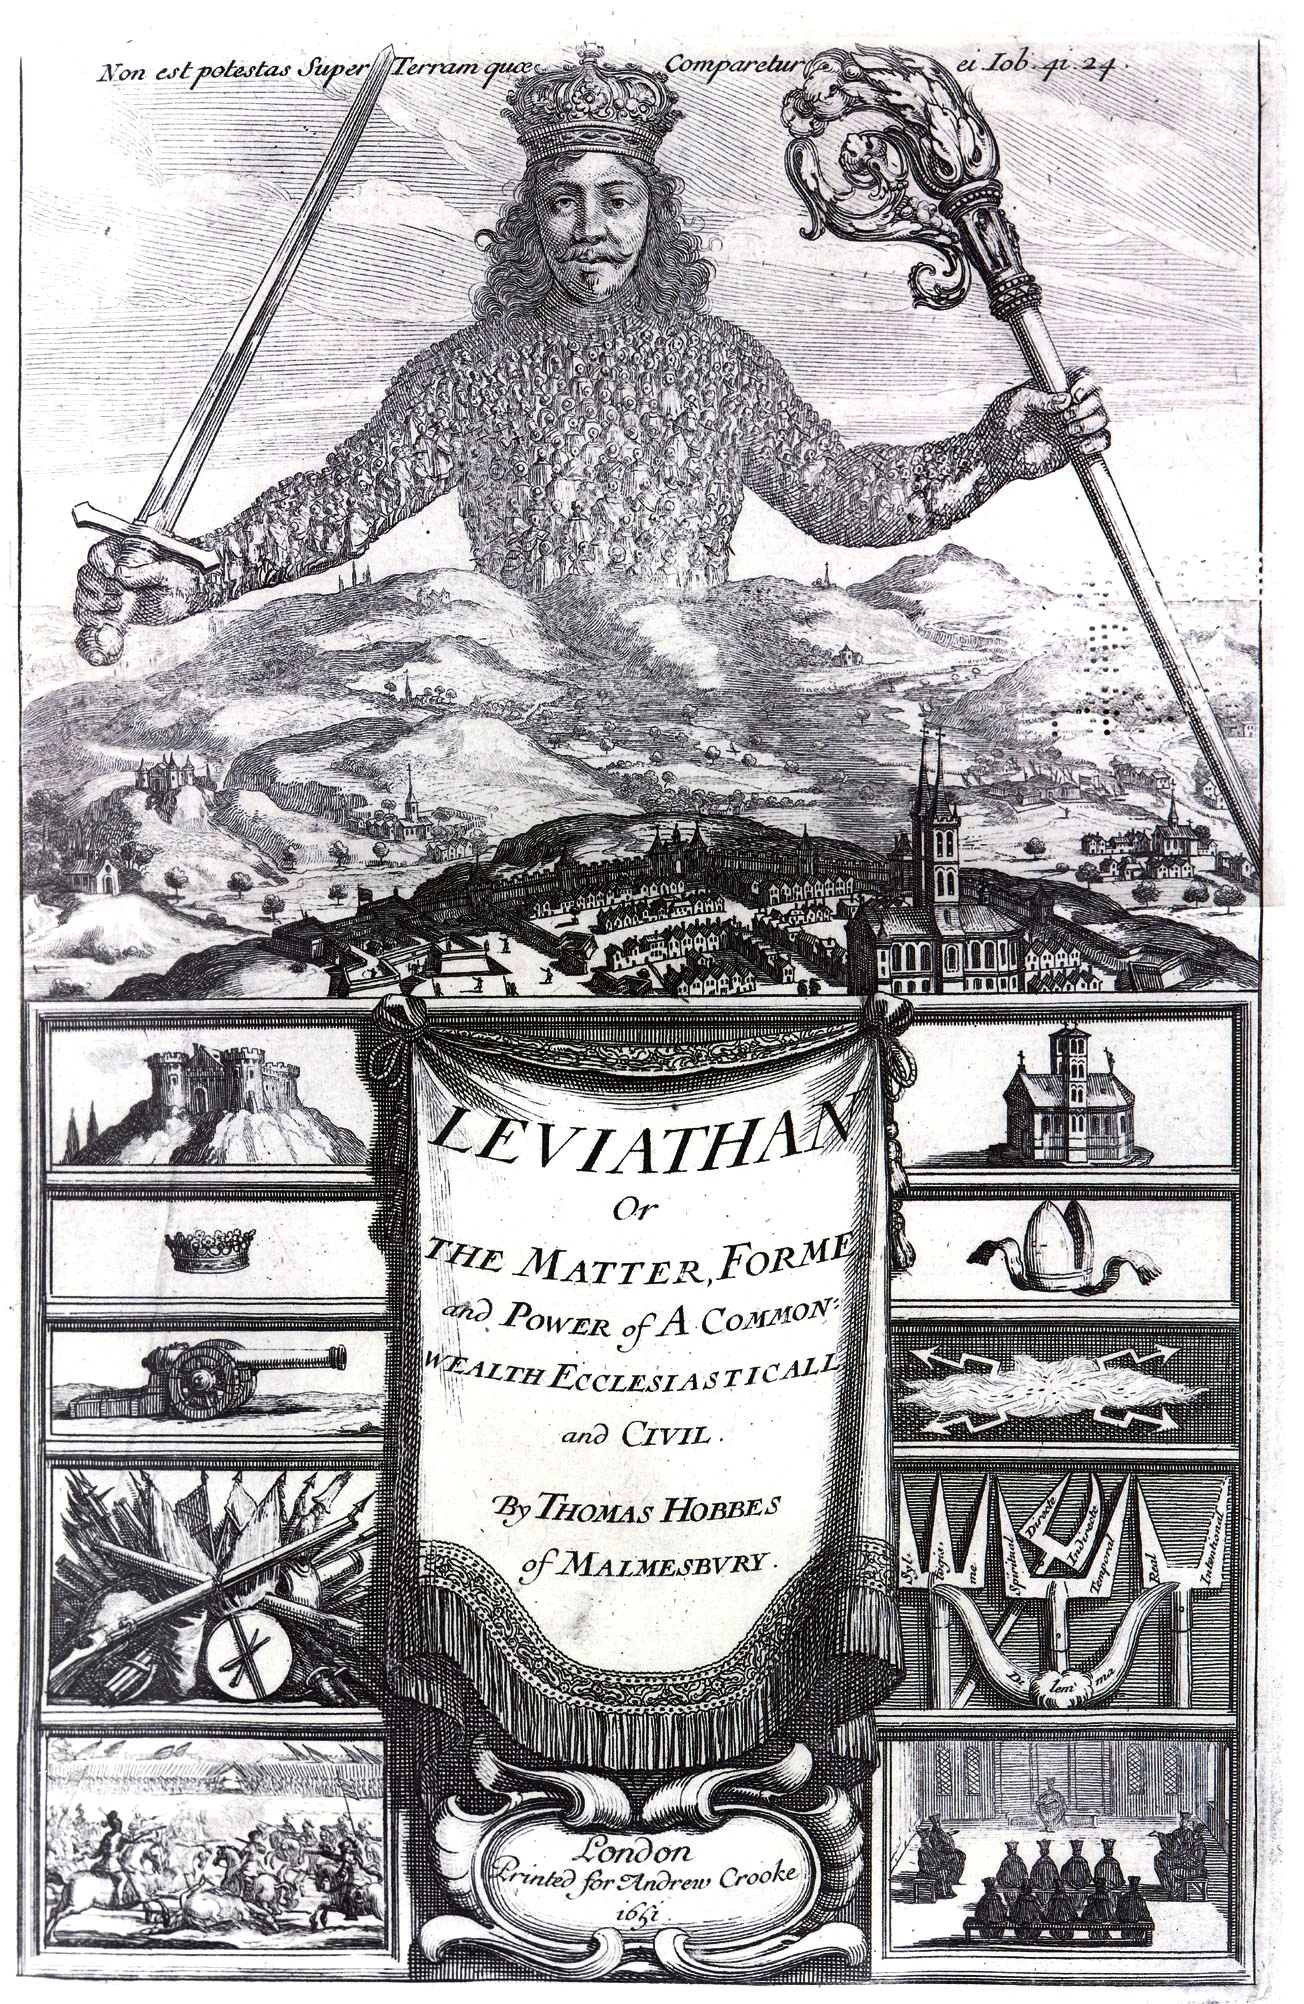
\includegraphics[width=50mm]{images/leviathan.jpg}
    \caption{『リヴァイアサン』表紙}
  \end{figure}



\newpage{}






\section{ロック『統治二論』(『市民政府論』)(1690)}


 % \begin{wrapfigure}{r}{60mm}
 %   \begin{center}
 %     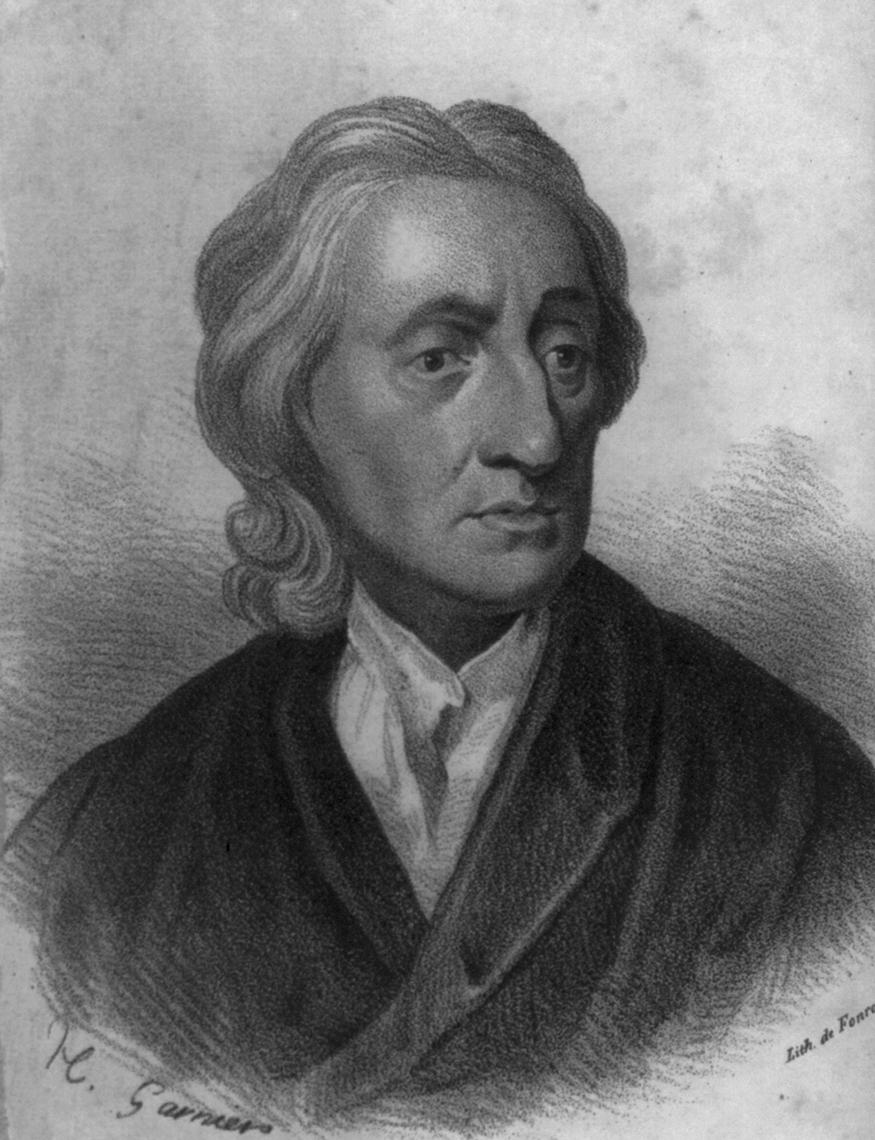
\includegraphics[width=50mm]{images/Locke-John-LOC.jpg}
 %     \caption{ロック} 
 %   \end{center}
 % \end{wrapfigure}


ジョン・ロック (John Locke, 1632--1704)。


典拠:ジョン・ロック、『完訳 統治二論』、加藤節訳、岩波書店、2010。


\subsection{}


政治権力を正しく理解し、それをその起源から引き出すためには、われわれは、すべての人間が自然にはどんな状態にあるかを考察しなければならない。それは、人それぞれが、他人の許可を求めたり、他人の意志に依存したりすることなく、自然法の範囲内で、自分の行動を律し、自らが適当と思うままに自分の所有物や自分の身体を処理することができる完全に自由な状態である。

それはまた、平等な状態であり、そこでは、権力と支配権とは相互的であって、誰も他人以上にそれらをもつことはない。なぜなら、同じ種、同じ等級に属する被造物が、すべて生まれながら差別なく同じ自然の便益を享受し、同じ能力を行使すること以上に明白なことはないのだから、それらすべての者の主であり支配者である神が、その意志の明確な宣言によってある者を他の者の上に置き、その者に、明示的な任命によって疑う余地のない支配権と主権とを与えるのでない限り、すべての者が従属や服従の関係をもたず、相互に平等であるべきだということはあきらかであるからである。(296)



 % \begin{figure}[htbp]
 %   \centering
 %     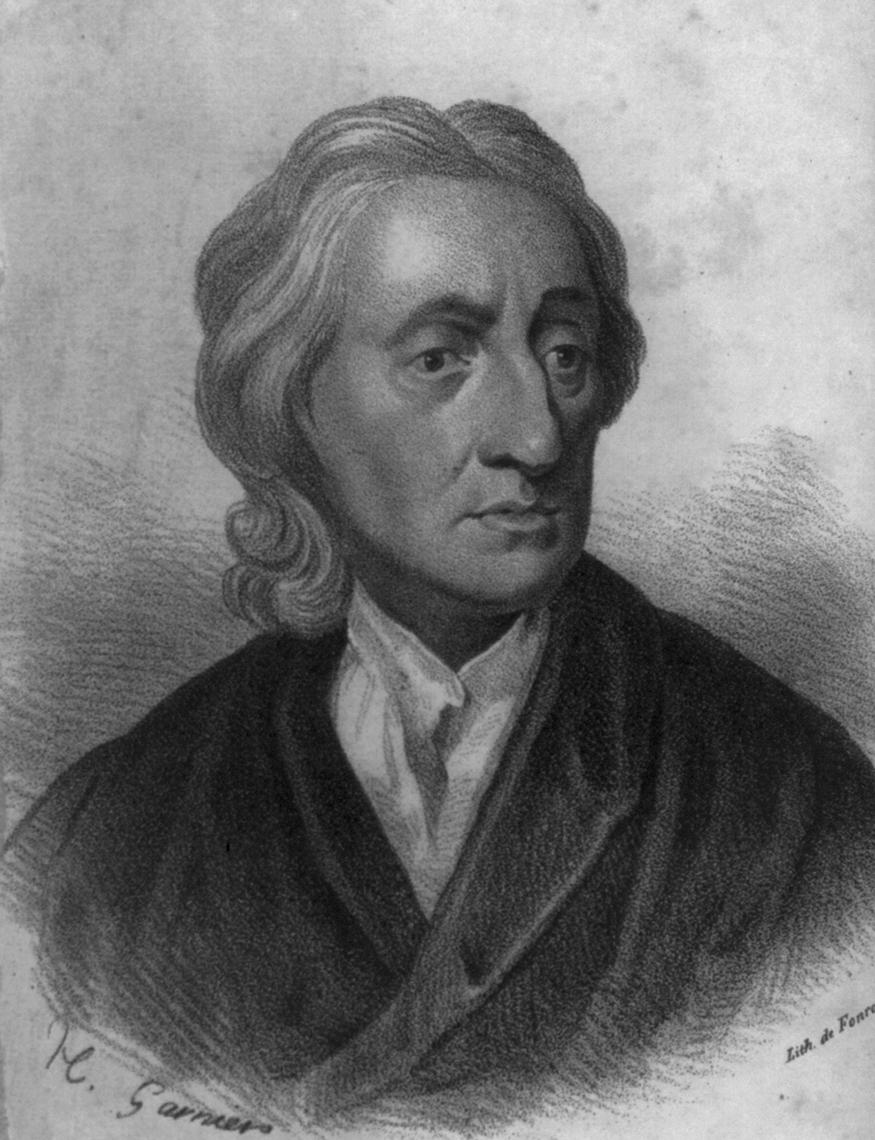
\includegraphics[width=50mm]{images/Locke-John-LOC.jpg}
 %   \caption{ロック}
 % \end{figure}


\begin{figure}[htbp]
  \centering
     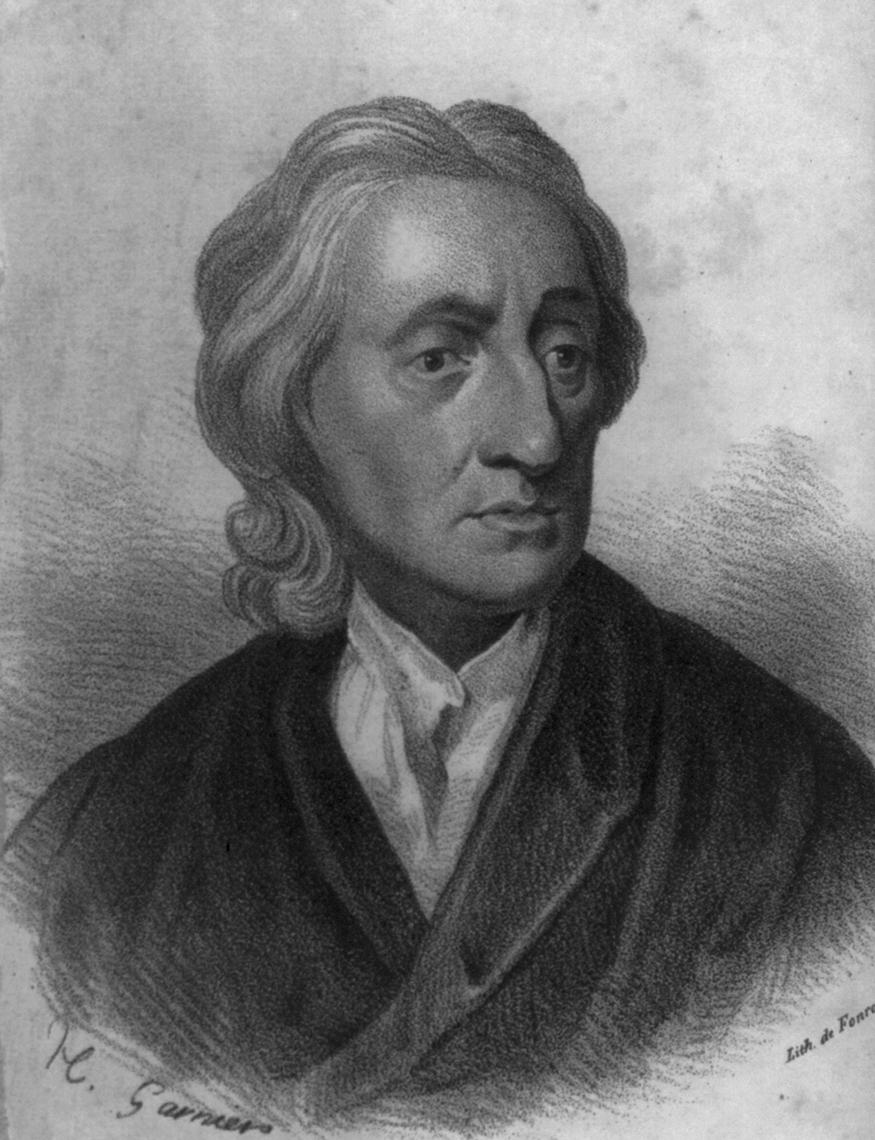
\includegraphics[width=50mm]{images/Locke-John-LOC.jpg}
     \caption{ロック} 

\end{figure}


\subsection{}


しかし、この自然状態は、自由の状態ではあっても、放縦の状態ではない。この状態において、人は、自分の身体と自分の所有物とを処理する何の制約も受けない自由をもっているにしても、彼は、自分自身を、また、自分が所有するいかなる被造物をも、単にその保全ということが要求する以上のより高貴な用途がある場合を除いて[ほしいままに]破壊する自由をもたないからである。自然状態はそれを支配する自然法をもち、すべての人間がそれに拘束される。そして、その自然法たる理性は、それに耳を傾けようとしさえすれば、全人類に対して、すべての人間は平等で独立しているのだから、何人も他人の生命、健康、自由、あるいは所有権を侵害すべきではないということを教えるのである。というのは、人間が、すべて、ただ一人の全能で無限の知恵を備えた造物主の作品であり、主権をもつ唯一の主の僕であって、彼の命により、彼の業のためにこの世に送り込まれた存在である以上、神の所有物であり、神の作品であるその人間は、決して他者の欲するままにではなく、神の欲する限りにおいて存続すべく造られているからである。そして、われわれは、同一の能力を授けられ、全員が一つの自然の共同体をなしているのだから、下級の被造物がわれわれのために造られているのと同じように、われわれも他人の用に供するために造られているかのように、相互に滅ぼし合うのを権威づけるような従属関係をわれわれの間に想定することはできない。各人は自分自身を保存すべきであり、勝手にその立場を放棄してはならないのだが、それと同じ理由から、自分自身の保全が脅かされない限り、できるだけ人類の他の人々をも保存すべきであり、また、侵害者に正当な報復をなす場合を除いては、他人の生命、あるいはその生命の維持に役立つもの、すなわち、自由、健康、四肢あるいは財貨を奪ったり、損ねたりしてはならないのである。

\subsection{}



そして、他人の権利を侵害したり、相互に危害を加えたりすることがないように万人を抑制し、平和と全人類の保存とを欲する自然法が遵守されるように、自然状態においては、自然法の執行は各人の手に委ねられているのであり、これによって、各人は、この法に違反する者を、法の侵害を防止する程度にまで処罰する権利をもつ。なぜならば、もし自然状態において自然法を執行する権力をもち、それによって無実の者を保全し、違反者を抑制する者がいないとすれば、自然法は、この地上の人間に関係する他のすべての法と同様に、空しいものになってしまうであろうからである。また、この自然状態において、誰かが自分に悪をなした者を処罰してもよいとすれば、すべての者がそうしてもよいということになるであろう。というのは、本来的に、一人の人間の他の人間に対する優位性や支配権が存在しないこの完全に平等な状態にあっては、ある者が、自然法を執行するためになしうることは、何人も、当然に、同様のことをなしうる権利をもっていなければならないからである。(298-300)

\subsection{}



人間に世界を共有物として与えた神は、また、彼らに、世界を生活の最大の利益と便宜とになるように利用するための理性をも与えた。大地と、そこにあるすべてのものとは、人間の生存を維持し快適にするために与えられたのである。そして、大地が自然に生みだす果実や大地が養う獣たちは、すべて、自然の自ずからなる手によって産出されたものであるから、人類に共有物として帰属し、従って、それらがそうした自然状態にある限り、それらに対して、何人も他人を排除する私的な支配権を本来的にもちえない。しかし、それらは人間が利用するために与えられたのだから、それらが、何かに利用される前には、あるいは、誰か特定の人にとって有益なものになるに先立って、何らかの方法でそれらを専有する手段が必ずやあるに違いない。囲い込みを知らず、今なお共有地の借地人である未開のインディアンを養う果実や鹿の肉は、それらが実際に彼らの生存を支えるために役立つものとなりうる前に、まず彼らのものであり彼の一部であって、他の者がそれに対してはいかなる権利をももちえないものでなければならない。

\subsection{}

たとえ、大地と、すべての下級の被造物とが万人の共有物であるとしても、人は誰でも、自分自身の身体に対する固有権〔プロパティ〕をもつ。これについては、本人以外の誰もいかなる権利をももたない。彼の身体の労働と手の働きとは、彼に固有のものであると言ってよい。従って、自然が供給し、自然が残しておいたものから彼が取りだすものは何であれ、彼はそれに自分の労働を混合し、それに彼自身のものである何ものかを加えたのであって、そのことにより、それを彼自身の所有物とするのである。それは、自然が設定した状態から彼によって取りだされたものであるから、それには、彼の労働によって、他人の共有権を排除する何かが賦与されたことになる。というのは、この労働は労働した人間の疑いえない所有物であって、少なくとも、共有物として他人にも十分な善きものが残されている場合には、ひとたび労働が付け加えられたものに対する権利を、彼以外の誰ももつことはできないからである。(325-326)









\subsection{}






すでに述べたように、人間はすべて、生来的に自由で平等で独立した存在であるから、誰も、自分自身の同意なしに、この状態を脱して、他者のもつ政治権力に服することはできない。従って、人々が、自分の自然の自由を放棄して、政治社会の拘束の下に身を置く唯一の方法は、他人と合意して、自分の固有権〔プロパティ〕と、共同体に属さない人に対するより大きな保障とを安全に享受することを通じて互いに快適で安全で平和な生活を送るために、一つの共同体に加入し結合することに求められる。この合意は、どれだけの人数の人間によってもなされることが許されるであろう。彼らは、それによって、自然状態の自由のうちにとどまる他の人間の自由を侵害することはないからである。こうして、どれだけの数の人間であろうと、人々が一つの共同体あるいは統治体を作ることに合意した場合、彼らは、それによって直ちに結合して一つの政治体をなすことになり、しかも、そこでは、多数派が決定し、それ以外の人々を拘束する権利をもつのである。

\subsection{}




というのは、ある数の人々が、各個人の同意によって一つの共同体を作った場合、彼らは、それによって、その共同体を一体となって行動する権力をもつ団体としたのであり、しかもそうした行動は、多数派の意志と決定とによらない限り不可能であるからである。つまり、ある共同体を動かすのはそれを構成する各人の同意であり、一つの団体は一つの方向に動く必要があるのだから、その団体は、より大きな力、すなわち多数派の同意が導く方向に進まなくてはならない。そうでなければ、それは、一つの団体、一つの共同体として行動することも存続することもできないであろう。これこそが、その共同体へと結合した各個人がそうあるべきだとして同意したことなのだから、各人は、その同意によって、多数派の拘束を受けなければならないのである。われわれが目にするように、実定法によって行動する権限を与えられているいかなる集合体においても、その実定法が特に数を定めていない場合には、多数派の決議が全体の決議として通用し、また、それが、自然と理性との法によって全体の権力を当然に決定するとされるのはそのために他ならない。(406-407)

\subsection{}


人々が社会に入る理由は、彼らの固有権〔プロパティ〕を保全することにある。そして、彼らが立法部を選出し、彼らに権威を与える目的は、その社会の全成員の固有権〔プロパティ〕に対する監視役あるいは防壁として、社会の各部分、各成員の権力を制限し、その統治権を適度に抑えるために法を作り、規則を定めることにある。なぜならば、立法部は、各人が社会に入ることによって確保しようと意図したもの、そのためにこそ人民が自分たちで作りだした立法者に服しているものを破壊する権力をもつべきだなどということが社会の意志であるとはとうてい考えられないので、立法者が、人民の固有権〔プロパティ〕を奪い、また破壊しようとするとき、あるいは、人民を恣意的な権力に服する隷属状態へと追いやろうとするときには、立法者は常に人民との戦争状態に置かれることになり、それによって、人民はもはやそれ以上のいかなる服従からも解放されて、神が力と暴力とに備えて万人のために用意した共通の避難所へと身を委ねることになるからである。従って、立法部が、社会のこの基本的な規則に違反し、野心や恐怖や愚かさや堕落によって人民の生命、自由、資産に対する絶対的な権力を自ら握ろうとしたり、あるいは誰か他人の手に置こうとしたりする場合にはいつでも、立法部は、この信託違反によって、人民がまったく異なった目的のために立法部の手に置いた権力を喪失し、人民にその権力が復帰することになろう。人民は、彼らの根源的な自由を回復する権利をもち、(自分たちが適当と思うような)新たな立法部を設立することによって、彼らが社会のうちに身を置く目的である自分自身の安全と保護とに備える権利をもつからである。そして、私がここで立法部一般について述べたことは、最高の執行権者についてもまたあてはまるであろう。つまり、彼は、立法部に関わり、法の最高の執行に関わるという二重の信託を受けているのだから、彼は、自分自身の恣意的な意志を社会の法として打ちたてようとする場合には、それら二つの信託に違反して行動することになるのである。更に、彼は、社会の武力や財や官職を利用して代表者たちを買収し、彼らを自分の目的のために抱きこむ場合や、彼が、公然と事前に選挙人と約束を交わして、懇願、脅迫、約束その他の方法によって自分の目的に抱きこんでおいた者を選ぶように指図したり、何に投票し、いかなる法を制定するかを前もって約束した人々を送り込むために選挙人を使ったりする場合にも、信託に違反して行動することになろう。このように候補者や選挙人を統制し、選挙の方法の新しいモデルを定めるということは、統治をその根底から断ち切り、公共の安全の源泉そのものに毒を投げ込むこと以外の何ものでもない。なぜならば、自分自身の固有権〔プロパティ〕の防壁として、代表者の選択権を保持している人民にとって、その権利を行使する目的は、代表者が常に自由に選ばれ、そのように選ばれた後は、吟味と十分な討論とを経た上で、政治的共同体の必要性と公共の善とにとって求められるものだと判断したところに従って、彼らに自由に行動してもらい、助言を与えてもらうこと以外にはないからである。討論を聴き、あらゆる面から道理を考慮する前に投票してしまう人に、それができるはずはない。人民の真の代表者や社会の立法者の代わりに、このような議会を準備し、自分自身の意志の公然たる推進者を押したてようとすることは、確かに、遭遇しうる限りでの最大の信託違反であり、統治を転覆しようとする企図のもっとも完全な宣言に他ならない。その上、人が、同じ目的のために公然たる賞罰を加えたり、そうした企図の前に立ちふさがり、祖国の自由を裏切ることに応じたり同意を与えたりしない人々を排除し撲滅するために、法を逆用した術策を用いたりするとき、そこで何が行われようとしているかについては疑問の余地がないであろう。権力が最初に設定されたときに、それに随伴した信託に反して権力を用いる者が、社会のなかでいかなる権力をもつべきであるかは容易に決定される。そうしたことを企てる人間がもはや信頼するに値しないということは、誰しも認めざるをえないであろう。(560-563)




\section{ルソー『社会契約論』 (1762)}

ジャンジャック・ルソー (Jan-Jacques Rousseau, 1712--1778)。

典拠:ジャン=ジャック・ルソー、『社会契約論』、作田啓一訳、白水社、2010。

\subsection{第一篇の主題}



 % \begin{wrapfigure}{r}{60mm}
 %   \begin{center}
 %     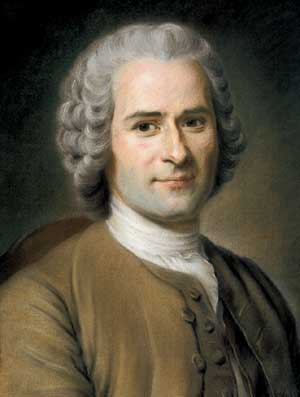
\includegraphics[width=50mm]{images/rousseau.jpg}
 %     \caption{ルソー} 
 %   \end{center}
 % \end{wrapfigure}


人間は自由なものとして生まれたが、しかもいたるところで鉄鎖につながれている。他の人々の主人であると信じている者も、その人々以上に奴隷であることを免れてはいないのだ。このような変化がどうして起こったのか。私にはわからない。それは何によって正当化されえているのか。私はこの問いなら解きうると思う。

もし私が、力と、力から生ずる結果とだけしか考慮しないとすれば、私はこう言うだろう。「ある人民が服従を強いられ、またじっさいに服従しているあいだは、それでよい。人民がその軛を振りほどくことができるようになり、またじっさいに振りほどくやいなや、なおさらよい状態となる。なぜなら、人民から自由を奪ったのとまったく同じ権利によって、人民は自由を回復したのである以上、人民が自由を奪い返すのは当然であるか、それとも、人民から自由を奪うのはもともと不当であったのか、そのどちらかであるからだ」と。しかし、社会秩序は神聖な権利であり、他のあらゆる権利の基礎として作用する。ところが、この権利は自然から出てくるものではなく、したがって、いくつかの約束にもとづくものである。問題は、これらの約束がどんなものかを知ることだ。(12)

 \begin{figure}[htbp]
   \centering
     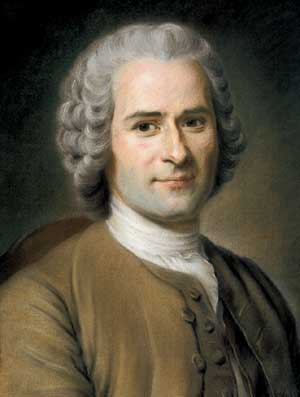
\includegraphics[width=50mm]{images/rousseau.jpg}
   
   \caption{ルソー}
 \end{figure}



\subsection{社会契約について}



各個人が自然状態にとどまろうとして用いる力よりも、それにさからって自然状態のなかでの自己保存を妨げる障害のほうが優勢となる時点まで、人間が到達した、と想定してみよう。そのとき、この原始状態はもはや存続しえなくなる。だから、もし生存様式を変えないなら、人類は滅びるだろう。

ところで、人間は新しい力をつくりだすことはできず、現に持っている諸力を結びつけ、方向を与えることができるだけであるから、生き残ってゆくためには、障害の抵抗に打ち勝てるようにみなが集まって諸力の総和をつくりだし、これらの力をただ一つの原動力で動かして、共同の活動に向けることしか、ほかに方法はない。

この力の総和は、多くの人たちの協力によってしか生じえない。ところが、各人の力と自由は、それぞれの人の生存にとっての第一の手段である。それでは、どのようにして、各人が損失をこうむることもなく、自分に向けられる当然の配慮をおろそかにすることもなしに、自分の力と自由をささげうるのだろうか。この難点は、私の主題に置き直すと、次の言葉で言いあらわすことができる。

「各構成員の身体と財産とを、共同の力のすべてを挙げて防衛し保護する結社形態を発見すること。そして、この結社形態は、それを通じて各人がすべての人と結びつきながら、しかも自分自身にしか服従せず、以前と同じように自由なままでいられる形態であること」。これこそ根本的な問題であり、社会契約がそれに解決を与える。

この契約の諸条項は、その結社行為の本性そのものから導かれているので、少しでも修正すれば、無意味で無効なものになってしまう。だから、これらの条項は、おそらく成分で言いあらわされたことはなかったとしても、どこにおいても同一であり、どこにおいても暗黙のうちに受け入れられ、承認されている。社会契約が破られて、各人が自分の最初の権利に立ち返り、約束によって得た自由を失うことによって、その自由を得るために放棄していた自然的自由を取り戻すまでは。

これらの諸条項は、よく考えてみれば、すべてがただ一つの条項に帰着する。すなわち、各構成員は自分の持つすべての権利とともに自分を共同体全体に完全に譲渡することである。というのは、第一に、各人は自分のいっさいを与えるのだから、すべての人にとって条件は等しく、また、条件がすべての人にとって等しいのだから、だれも他人の負担を重くすることに関心を抱かないからである。

そのうえ、この譲渡は保留なしに行なわれるので、結合〔アソシアシオン〕はこのうえもなく完全であり、どの構成員も、もはや要求するものをなに一つ持たない。なぜなら、もし、諸個人になんらかの権利が残されるとすれば、彼らと公衆〔=人民〕とのあいだに立って裁きをつけることができるような共通の上位者はだれもいない以上、各人はある点で自分自身の裁判官であることになり、やがては、あらゆることについて裁判官であることを主張するようになるからである。そうなると、自然状態が存続することになり、結社は必然的に圧政的になるか、空虚なものとなるだろう。

要するに、各人はすべての人に自分を与えるから、だれにも自分を与えないことになる。そして、各構成員は自分に対する権利を他人に譲り渡すか、それと同じ権利を他人から受け取らないような構成員はだれもいないのだから、人は失うものと等価のものを手に入れ、また、持っているものを保存するための力を〔結社によって〕より多く手に入れるのである。

そこで、もし社会契約から、本質的でないものを取り除くなら、次の言葉に帰着することがわかるだろう。われわれのおのおのは、身体とすべての能力を共同のものとして、一般意志の最高の指揮のもとに置く。それに応じて、われわれは、団体のなかでの各構成員を、分割不可能な全体の部分として受け入れる。

この結社行為は、直ちに各契約者の個々の人格に代わって、ひとつの精神的で集合的な団体を生みだす。その団体は、〔これを設立する〕集会の有する投票権と同数の成員からなり、この同じ結社行為から、その統一、その共同の自我、その生命、その意志を受け取る。このように、おのおのの個人がすべての他者と結びつくことによって形成されるこの公的人格は、かつては都市〔国家〕(Cité)いまは共和国(Répblique)または政治体(corps politique)と名づけられている。それが動的な面でとらえられる場合は、その成員によって国家(Etat)と呼ばれ、能動的な面でとらえられる場合は、主権者(Souverain)と呼ばれる。他の同様の公的人格とくらべるときは、国(Puissance)と呼ばれる。構成員について言えば、集合的には人民(peuple)という名称を持ち、主権者として参加する個々の単位としては市民(Citoyens)、国家の法に従うものとしては臣民〔=被治者〕(Sujets)と呼ばれる。しかし、これらの用語はしばしば混同され、互いに取り違えられている。ただ、これらの用語を完全に正確に使おうとする場合に、それらを区別できれば、それで十分である。(26-29)

\subsection{主権者について}



この公式から次のことがわかる。結社行為は、公衆〔=人民〕と個々人とのあいだの約束を含むこと、また各個人は、いわば自分自身と契約しているので、二重の関係で{\——}すなわち、主権者の成員としては個々人に対して、国家の成員としては主権者に対して{\——}約束していることになる。しかし、何びとも自分自身と結んだ約束には拘束されないという民法の格率は、ここでは適用できない。というのは、自分に対して義務を負うことと、自分がその一部分を成している全体に対して義務を負うこととのあいだには、大きな相違があるからである。

なお、次のことに注意しておかなければならない。すなわち、臣民〔=被治者〕の一人一人は〔前節で述べたように〕二つの異なった関係から考察されているから、公共の議決が、彼らのすべてを主権者に対して義務づけることができるが、その理屈を逆に使って、この議決が主権者を主権者自身に対して義務づけることはできない、ということ、したがってまた、主権者がみずから破ることのできない法を自分に課するのは、政治体の本性に反する、ということである。主権者は一つの同じ関係からしか自分自身を考えることができないのだから、その状況は、自分自身と契約する個々人の場合と同じである。そこから、人民という団体に義務を負わすいかなる種類の基本法もなく、またありえないことがわかる。社会契約でさえも同様である。このことは、その団体が、社会契約に違反しない事柄においても、他者〔=外国〕としっかりした約束を結べないということを意味するものではない。なぜなら、外国に対しては、この団体は単一の存在、一個人となるのだから。

しかし、政治体または主権者は、ひとえに神聖な契約によって存立しているのであるから、他者〔=外国〕に対してさえ、この原初の行為に違反するようなことで、何一つ自分を縛ることはできない。たとえば、自分自身のどこか一部分を譲渡するとか、他の主権者に服従するといったことである。自分が存立する根拠となった〔約束〕行為に違反すると、みずからの滅亡にいたるだろう。そして、無にすぎないものは何ものも生みださない。

群衆がこのように集合して一つの団体をつくるやいなや、一人でもその成員を傷つければ、かならず団体を攻撃したことになるし、まして団体を傷つければ、かならず成員たちの怨みを買うことになる。こういうわけで、義務と利益とが等しく双方の契約当事者を縛り、相互に助け合うようにさせる。そして、同じ人々が、この二重の関係のもとで相互扶助にもとづくあらゆる利点を結びつけようと努めるに違いない。

ところで、主権者はそれを構成している個々人からのみ成り立っているのであるから、彼らの利益に反する利益を持っていないし、また持つこともできない。したがって、主権者の権力はその臣民に対して、なんらの保証を与える必要はない。政治体がその全成員を害しようと欲することはありえないからである。そして、後述するように、政治体は個人としての何びとをも害することはできない。主権者は、ただ存在するということだけで、つねに主権者たる要件をすべて備えている。

しかし、臣民が主権者に対する場合は、こうはいかない。その場合には、〔約束を守るのが〕臣民の共同の利益であるにもかかわらず、主権者が臣民の忠誠を確保する方法を見いださないかぎり、彼らが約束を守るかどうかの保証はどこにもない。

じっさい、人間としての各個人は、市民としての彼の持っている一般意志に反したり、あるいはそれと異なる特殊意志を持つことがある。彼の特殊意志は、共同の利益とはまったく違ったふうに彼に話しかけることがある。人間はだれでも絶対的な存在であり、本来は独立した存在であるから、共同の利益のために課せられている義務の遂行を無償の寄付であるとみなし、自分にとって高くつく支払いにくらべれば、〔寄付をしないことで〕他人の受ける損失のほうが少ないと考えることもありうる。そして、彼は、国家を構成する精神的人格が一個の人間ではないという理由から、これを理屈で考え出したものとみなし、臣民の義務を果たそうともしないで、市民の権利を享受するかもしれない。このような不正が進めば、政治体の破滅を招くだろう。

したがって、社会契約を空虚な公式としないために、一般意志への服従を拒む者はだれでも、団体全体によって服従を強制される、という約束を暗黙のうちに含んでいるのであり、そして、この約束だけが、他の約束に効力を与えうるのである。このことはただ、彼が自由であるように強制される、ということを意味しているにすぎない。なぜなら、このようなことこそ、各市民を祖国にゆだねることによって彼をすべての個人的依存から守護する手段であり、政治機構の装置と運動を生みだす条件であり、市民のあいだのさまざまな約束を合法的なものとする唯一の条件であるからだ。この条件がなければ、これらの約束は、不条理で圧政的なものとなり、大変な誤用に陥るだろう。(30-33)

\subsection{社会状態について}



自然状態から社会状態へのこの推移は、人間のうちにきわめて注目すべき変化をもたらす。というのは、人間の行為において、正義を本能に置きかえ、これまで欠けていた道徳性を人間の行為に与えるからである。そのときにはじめて、義務の呼び声が肉体の衝動に、権利が欲望にとって代わり、そのときまでは自分のことしか考えていなかった人間が、以前とは別の原理によって動き、自分の好みに耳を傾けるまえに理性に問い合わせなければならなくなっていることに気づく。この状態において、彼は自然から受けていた多くの利益を失うとしても、その代わりきわめて大きな利益を手に入れる。彼の能力は訓練されて発達し、彼の考えは広がり、彼の感情は気高くなり、彼の魂全体が高められる。このような高所に達するので、もしこの新しい状態の悪用のために、彼が脱出してきたもとの状態以下に堕落するようなことがなければ、彼をもとの状態から永久に引き離し、愚かで視野の狭い動物を知性的存在でありかつ人間たらしめたあの幸福な瞬間を、彼はたえず祝福しなければならないだろう。

この特質の総決算を比較しやすい項目で要約してみよう。人間が社会契約によって失うもの、それは彼の自然的自由と、彼の欲望を誘い、しかも彼が手に入れることのできるすべてのものに対する無制限の自由とである。これに対して彼がかち得るもの、それは社会的自由〔リベルテ・シヴィル〕と、彼が持っているすべてのものに関する所有権とである。この埋め合わせについて思い違いをしないためには、もっぱら個人の力だけが限度を左右する自然的自由と、一般意志によって制限されている社会的自由との違いを、はっきり見分けることが必要だ。また、暴力の結果か先占権にすぎない占有と、法律上の権原にもとづいてはじめて成り立ちうる所有権との違いを、はっきり見分けることが必要だ。

上に述べたところにもとづき、人間を真にみずからの主人たらしめる唯一のもの、すなわち道徳的自由を、社会状態において獲得するもののなかにつけ加えることができよう。なぜなら、欲望だけにかりたてられるのは奴隷状態であり、みずから課した法に従うことが自由だからである。しかし、私はこの問題についてもう十分過ぎるほど語ったし、また、自由という語の哲学的意味は私の課題ではない。(34-35)

\subsection{第二篇}



全体意志と一般意志とのあいだには、しばしばかなり相違がある。後者は共同の利益だけを考慮する。前者は私的な利益にかかわるものであり、特殊意志の総和にすぎない。しかし、これらの特殊意志から、〔一般意志との距離である〕過不足分を相殺させて引き去ると、差の総計が残るが、これが一般意志である。

人民が十分な情報をもって討議するとき、もし、市民相互があらかじめなんの打ち合わせもしていなければ、〔一般意志との〕わずかな差が多く集まって、その結果つねに一般意志が生み出されるから、その結果はつねによいものであろう。ところが、部分結社である徒党が、大結社〔=政治体〕を犠牲にしてつくられると、これらの部分的結社のおのおのの意志は、その構成員に対しては一般的であるが、国家に対しては特殊的となる。その場合には、もはや人々と同じ数の投票者があるのではなくて、部分的結社と同じ数の投票者があるにすぎなくなると言えよう。差の数が減少すると、その結果として一般性の程度も減少する。ついには、これらの結社の一つが非常に大きくなって、他のすべての結社を圧倒するようになると、結果は、もはやさまざまのわずかな差の総和があるのではなく、ただ一つの差だけがある、ということになる。そうなれば、もはや一般意志は存在せず、勝利を占める意見は、特殊な意見であるにすぎない。

それゆえ、一般意志が十分に表明されるためには、国家の中に部分社会が存在せず、おのおのの市民が自分だけに従って意見を述べることが必要である。偉大なリュクルゴスの独特で卓抜な制度はこのようなものであった。いくつかの部分社会があるときには、ソロン、ヌマ、セルヴィウスの行なったように、その数をふやし、その間の不平等を防止しなければならない。こうした周到な用意こそ、一般意志がつねに輝きを失わず、人民が誤りを犯さないための唯一の良策なのである。(46-48)


法律とは、本来社会的結合〔アソシアシオン・シヴィル〕の諸条件以外の何ものでもない。法律に従う人民が法律の作成者でなければならない。社会の諸条件を規定する権限は、結合している人々だけに属する。しかし、彼らはどのようにして規定をつくるだろうか。〔……〕人民は、おのずから、いつも幸福〔ビアン〕を求めてはいるが、何が幸福かを、いつもひとりでにさとるとはかぎらない。一般意志はつねに正しいが、それを導く判断はつねに啓蒙されているわけではない。一般意志に、対象をあるがままの姿で、ときにはあるべき姿で見させることが必要である。一般意志に、それが求めている正しい道を示し、特殊意志の誘惑から守り、所と時に注意を向けさせ、目前の感知しやすい利益の魅力と、遠くにあって隠れている災いの危険とを、秤にかけて示してやることが必要である。個々人は幸福がわかっていても、これを退け、公衆は、幸福を欲していても、それがわからない。両者とも等しく導き手が必要なのである。個々人については、彼らの意志を理性に一致させるよう強制しなければならないし、公衆については、彼らが欲しているものを教えてやらなければならない。こうして、公衆が啓蒙されると、社会全体のなかに悟性と意志との一致が生まれ、そこから諸部分の緊密な協力が生じ、ついには全体としての最大の力が発動する。こういうわけで、立法者が必要となってくるのである。(61-62)


あらゆる体系的立法の目的であるべき、すべての人々の最大の福祉とは、正確には何から成り立っているかを探求してゆくと、われわれはそれが二つの主要な目標、すなわち自由と平等とに帰着することがわかるだろう。なぜ自由なのか。特殊なもの〔=個人または徒党〕への依存はどのようなものであれ、すべて国家という〔政治〕体から、それだけ力を奪うことになるから。なぜ平等なのか。それがなければ自由は存続しえないから。

社会的自由とは何かについてはすでに述べた。平等について見れば、この語を、権力と富の程度の絶対的な同一性の意味に解してはならないのであって、次のように理解しなければならない。すなわち、権力に関しては、それがどんなに強くても、暴力にまではいたらず、地位と法律によるのでなければけっして行使されてはならない、ということ。次に、富に関しては、いかなる市民も他の市民を買えるほど富裕ではなく、また、いかなる市民も身売りを余儀なくされるほど貧困であってはならない、ということ。そのためには、上層の側では財産と勢力を、下層の側では貪欲と羨望を、それぞれ抑制することが前提となる。(80-81)


\vspace{2zw}

\section{推薦図書}



\begin{itemize}
\item 田中浩(1998)『ホッブズ』、研究社出版。ホッブズの評伝。時代背景など非常にわかりやすい。(江)
\item 田中浩(2006)『ホッブズ』、清水書院。(渡)
\item 野田又夫 (1985)『ロック』、講談社。(渡)
\item 松下圭一 (1987) 『ロック「市民政府論」を読む』、岩波書店。昭和の偉い先生による一般読者市民向け解説。(江)
% \item 浜林正夫 (1996) 『ロック』、研究社出版。この「イギリス思想叢書」シリーズはどれもよい。(江)
\end{itemize}




%%% Local Variables:
%%% mode: japanese-latex
%%% TeX-master: "main_gendai"
%%% coding: utf-8
%%% End:
